\documentclass{standalone}

\usepackage[english]{babel}

% to define font size

\usepackage{ulem}
\usepackage{moresize}
\usepackage{anyfontsize}

% to use colors

\usepackage[dvipsnames]{xcolor}
\usepackage{MnSymbol}

% to use tikz and its libraries

\usepackage{tikz-timing}
\usepackage{tikz}

\usetikzlibrary{backgrounds}
\usetikzlibrary{positioning, calc, arrows, shapes, automata, petri, patterns,decorations.markings}
\usetikzlibrary{decorations.pathreplacing}

% to use tikzmark, to place and refer to marks outside the current figure

\tikzset{every picture/.style={remember picture}}

% styles for transitions

\tikzset{transition/.append style={fill=black!20, thick}}
\tikzset{transition/.append style={fill=black!20, thick}}

% styles for test and inhib arcs.

\tikzstyle{test}=[pre, *-]
\tikzstyle{inhib}=[pre, o-]

\usepackage{circuitikzgit}
\ctikzset{
  logic ports=ieee,
}

% Arrow positioning in a path

\tikzset{->-/.style={decoration={
  markings,
  mark=at position #1 with {\arrow{>}}},postaction={decorate}}}

\tikzset{-<-/.style={decoration={
  markings,
  mark=at position #1 with {\arrow{<}}},postaction={decorate}}}

% shift values

\newcommand{\outportshift}{0mm}
\newcommand{\outportidpshift}{0mm}

%%%%%%%%%%%%%%%%%%%%%%%%%%%%%%%%%%%%%%%%%%%%%%%%%%
%                  BEGIN DOCUMENT                %
%%%%%%%%%%%%%%%%%%%%%%%%%%%%%%%%%%%%%%%%%%%%%%%%%%

\begin{document}

\begin{circuitikz}

  \ctikzset{multipoles/dipchip/width=2.5}
  \ctikzset{multipoles/dipchip/pin spacing=.18}

  \node (pn) {
    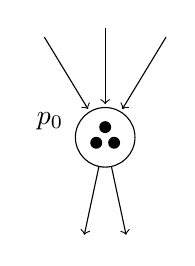
\begin{tikzpicture}

      % PLACES AND TRANSITIONS
      
      \node[place,tokens=3] (p0) {};
      
      % LABELS

      \node (pzLabel) at ($(p0)-(.7,-.2)$) { $p_0$};
      
      % ARCS
      
      \draw (p0) edge[pre] ($(p0.north west)-(.5,-1)$);
      \draw (p0) edge[pre] ($(p0.north)+(0,1)$);
      \draw (p0) edge[pre] ($(p0.north east)+(.5,1)$);
      % \node at ($(p0.north)+(0,1.2)$) {\dots};
      
      \draw (p0) edge[post] ($(p0.south west)-(0,1)$);
      \draw (p0) edge[post] ($(p0.south east)+(0,-1)$);
      % \node at ($(p0.south)-(0,1.2)$) {\dots};

    \end{tikzpicture}
  };
  
  % PCI idp
  
  % interface
  
  \draw       
  node [dipchip, num pins=26, hide numbers,
  no topmark, external pins width=0]
  (idp) at ($(pn.east)+(4,0)$) {$\gamma(p_0)$};

  \draw ($(idp.bpin 1)$)
  node [anchor=west, font=\ssmall] {\tt im}
  -- ++(-.3,0)
  node[anchor=east, font=\ssmall,xshift=\outportshift] {\tt \textcolor{blue}{3}};
  
  \draw ($(idp.bpin 2)$)
  node [anchor=west, font=\ssmall] {\tt iaw(0)} 
  -- ++(-.3,0);

  \draw ($(idp.bpin 3)$)
  node [anchor=west, font=\ssmall] {\tt iaw(1)}
  -- ++(-.3,0);

  \draw ($(idp.bpin 4)$)
  node [anchor=west, font=\ssmall] {\tt iaw(2)}
  -- ++(-.3,0);

  \draw [
    decorate, 
    decoration = {brace,
        raise=25pt,
        amplitude=3pt,
        aspect=0.5}] ($(idp.bpin 2)+(0,2pt)$) --  ($(idp.bpin 4)-(0,2pt)$)
      node[anchor=west,pos=.5,xshift=27pt]{\ssmall $=\vert\mathtt{input}(p_0)\vert$};

  \draw ($(idp.bpin 5)$)
  node [anchor=west, font=\ssmall]  {\tt itf(0)}
  -- ++(-.3,0);

  \draw ($(idp.bpin 6)$)
  node [anchor=west, font=\ssmall]  {\tt itf(1)}
  -- ++(-.3,0);

  \draw ($(idp.bpin 7)$)
  node [anchor=west, font=\ssmall]  {\tt itf(2)}
  -- ++(-.3,0);
  
  \draw ($(idp.bpin 8)$)
  node [anchor=west, font=\ssmall]  {\tt oat(0)}
  -- ++(-.3,0) coordinate (idpoat0);

  \draw ($(idp.bpin 9)$)
  node [anchor=west, font=\ssmall]  {\tt oat(1)}
  -- ++(-.3,0);

  \draw ($(idp.bpin 10)$)
  node [anchor=west, font=\ssmall]  {\tt oaw(0)}
  -- ++(-.3,0);

  \draw ($(idp.bpin 11)$)
  node [anchor=west, font=\ssmall]  {\tt oaw(1)}
  -- ++(-.3,0);

  \draw [
  decorate, 
  decoration = {brace,
    raise=25pt,
    amplitude=3pt,
    aspect=0.5}] ($(idp.bpin 10)+(0,2pt)$) --  ($(idp.bpin 11)-(0,2pt)$)
  node[anchor=west,pos=.5,xshift=27pt]{\ssmall $=\vert\mathtt{output}(p_0)\vert$};
  
  \draw ($(idp.bpin 12)$)
  node [anchor=west, font=\ssmall]  {\tt otf(0)}
  -- ++(-.3,0);

  \draw ($(idp.bpin 13)$)
  node [anchor=west, font=\ssmall]  {\tt otf(1)}
  -- ++(-.3,0);

  % Output port interface

  \draw ($(idp.bpin 23)$)
  node [anchor=east, font=\ssmall]  {\tt oav(0)}
  -- ++(.3,0);
  
  \draw ($(idp.bpin 22)$)
  node [anchor=east, font=\ssmall]  {\tt oav(1)}
  -- ++(.3,0);
  
  \draw ($(idp.bpin 21)$)
  node [anchor=east, font=\ssmall]  {\tt rtt(0)}
  -- ++(.3,0);

  \draw ($(idp.bpin 20)$)
  node [anchor=east, font=\ssmall]  {\tt rtt(1)}
  -- ++(.3,0);

  \draw ($(idp.bpin 19)$)
  node [anchor=east, font=\ssmall]  {\tt pauths(0)}
  -- ++(.3,0);

  \draw ($(idp.bpin 18)$)
  node [anchor=east, font=\ssmall]  {\tt pauths(1)}
  -- ++(.3,0);

  \draw ($(idp.bpin 17)$)
  node [anchor=east, font=\ssmall]  {\tt m}
  -- ++(.3,0);
  
  % generic map
  \node[anchor=north] at (idp.south) {\ssmall
    \begin{tabular}{@{}c@{}}
      ($\mathtt{ian}\Rightarrow\vert{}\mathtt{input}(p_0)\vert$), ($\mathtt{oan}\Rightarrow\vert\mathtt{output}(p_0)\vert$), \\
      ($\mathtt{mm}\Rightarrow{}b(p_0)$) \\
    \end{tabular}
  };

  \node at ($(pn.east)!.3!(idp.west)$) {\Huge$\rightarrow$};
  
\end{circuitikz}


\end{document}
%%% Local Variables:
%%% mode: latex
%%% TeX-master: t
%%% End:
